
\begin{figure}
	\begin{center}
		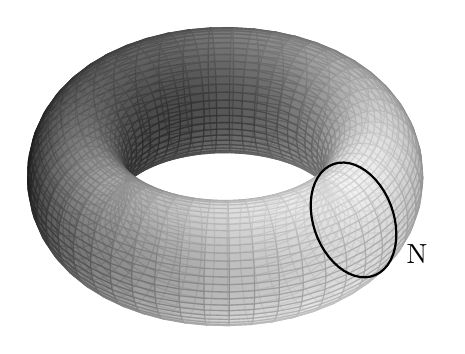
\begin{tikzpicture}[scale=1]
			\begin{axis}[
				colormap/blackwhite,
				view={30}{60},
				axis lines=none
				]
				% Plot the surface
				\addplot3[
				surf,
				opacity=0.7,
				samples=50,
				point meta=x+3*z*z-0.25*y,
				domain=0:2*pi,
				y domain=0:2*pi,
				z buffer=sort
				] 
				({(3+cos(deg(x)))*cos(deg(y))}, 
				{(3+cos(deg(x)))*sin(deg(y))}, 
				{sin(deg(x))});
				
				% Plot the vertical line
				\addplot3[
				domain=0:2*pi,
				samples=50,
				x=0,
				black,
				thick
				]
				({(3+cos(deg(x)))*cos(deg(0))}, 
				{(3+cos(deg(x)))*sin(deg(0))}, 
				{sin(deg(x))}) node[midway, below right] {N};
				
				
			\end{axis}
		\end{tikzpicture}
	\end{center}
\caption{In order to transition between states we need a loop of length {\bf N}}
\label{fig:Torus}
\end{figure}
